\chapter{Representación Vectorial de Palabras (Word Embeddings)}


\section{Introducción al concepto de \textit{Embedding}}

De manera intuitiva, un \textit{embedding} de texto es una representación matemática que proyecta un fragmento de texto en un espacio latente de alta dimensionalidad. En este espacio, la posición del texto se define mediante un vector, donde cada componente del vector corresponde a una dimensión. Al igual que en un plano cartesiano se tienen dos dimensiones, en un embedding, se suele trabajar con muchas más dimensiones para representar una palabra en el espacio\cite{henner_intuitive_embeddings_2023}. Por ejemplo, el modelo de \textbf{OpenAI} \textit{text-embedding-ada-002} el cual tiene un espacio de dimensión de 1536. Es decir, cada vector está formado por 1536 componentes.

Un ejemplo de cómo se verían los valores que toma cada dimensión es el siguiente:

\begin{quote}
  \textit{``A text embedding is a piece of text projected into a high-dimensional latent space. The position of our text in this space is a vector, a long sequence of numbers. Think of the two-dimensional cartesian coordinates from algebra class, but with more dimensions---often 768 or 1536.''} \cite{henner_intuitive_embeddings_2023}
\end{quote}

Al procesar el párrafo anterior mediante el modelo \textit{text-embedding-ada-002} mencionado, se obtiene la gráfica de la Figura \ref{fig:ejemploValoresEmbedding}, donde cada barra vertical representa el valor asignado a una de sus 1536 dimensiones.

\begin{figure}[h]
  \centering
  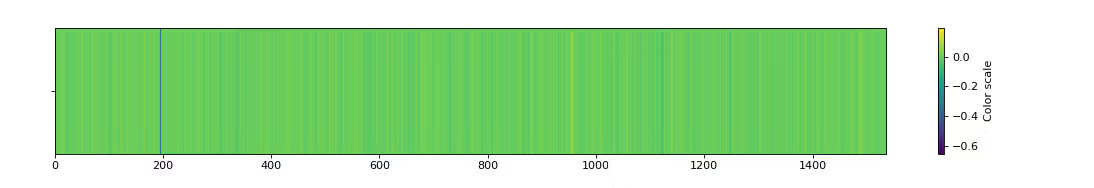
\includegraphics[width=0.8\linewidth]{imagenes/ejemploValoresEmbedding.png}
  \caption{Representación gráfica de los valores en las 1536 dimensiones de un embedding generado por el modelo text-embedding-ada-002. Fuente: \cite{henner_intuitive_embeddings_2023}.}
  \label{fig:ejemploValoresEmbedding}
\end{figure}

Un \textbf{espacio de embedding} o \textbf{espacio latente} se define matemáticamente como un espacio donde los elementos están posicionados de manera más cercana uno del otro cuando tienen valores parecidos, mientras que si difieren dichos elementos, se posicionan más lejos entre ellos. En el caso del \glsentrytext{pln}, frases que son semánticamente más similares a otras, tendrán un vector de embedding similar por lo que estarán más juntas en el espacio.

Aunque la comparación entre frases es una de las aplicaciones más conocidas, los \textit{embeddings} también se aplica en modelos de \glsentrytext{ml} y en arquitecturas de redes neuronales complejas.

\subsection{Embeddings de palabras (\textit{Word Embeddings})}

Mientras que el concepto general de \textit{embedding} puede aplicarse a frases completas (como en el ejemplo introducido), su uso más extendido e histórico se encuentra en su aplicación a nivel atómico: las palabras. Un \textit{embedding} de palabras, es un vector de longitud fija el cual su único cometido, es representar una única palabra o \textit{token} \cite{almeida_word_2023}.

El diseño y creación de estos vectores se clasifica principalmente en dos grandes familias estratégicas, dependientes de sus algoritmos de generación: los \textbf{modelos basados en predicciones} y los \textbf{modelos basados en conteos}.

\subsubsection{Modelos basados en predicciones}

Esta técnica de representación surgió fuertemente ligada al desarrollo de los \glsentryplural{mnl}. A diferencia de los enfoques estadísticos tradicionales de recuento, un modelo predictivo se centra en aprender el significado de un término de forma prospectiva, es decir, "adivinando".

Para lograrlo, emplean una red neuronal sencilla dotada de una ventana de contexto de tamaño fijo y móvil (por ejemplo, avanzando de cinco en cinco palabras). A medida que lee el texto, el modelo intenta predecir el significado de una palabra central en base a las palabras vecinas de esta ventana, o a la inversa, predecir el contexto apoyándose únicamente en dicho término central.

El aspecto fundamental en todo esto, es que tras finalizar el entrenamiento, el objetivo de \glsentrytext{ml} deja de ser la capacidad del modelo para adivinar con exactitud. En su lugar, de la red neuronal, se extraen los \textbf{pesos y valores} que ha ajustado internamente. Estos valores que fueron ajustados durante el entrenamiento, se convierten directamente en el \textit{word embedding}. En consecuencia, el mecanismo iterativo garantiza que aquellas palabras empleadas en contextos idénticos acaben reteniendo representaciones vectoriales prácticamente iguales.

\begin{figure}[h]
  \centering
  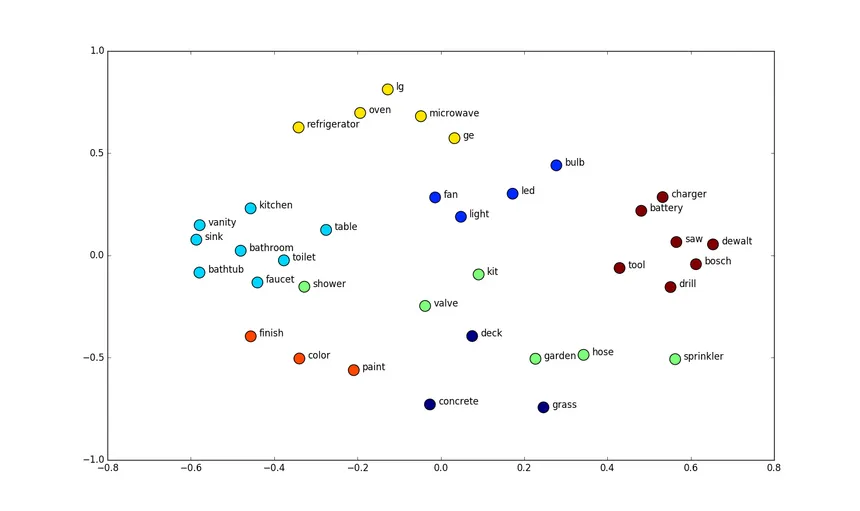
\includegraphics[width=0.8\linewidth]{imagenes/Word-embeddings-model.png}
  \caption{Representación visual de un modelo basado en predicciones para generar embeddings de palabras. Fuente: \url{https://neptune.ai/blog/word-embeddings-guide}.}
  \label{fig:word_embeddings_model}
\end{figure}

Una de las arquitecturas más representativas dentro de la predicción de \textit{embeddings} es la famosa familia algorítmica \textbf{Word2Vec}, la cual se detalla de forma exhaustiva en el próximo capítulo.

\subsubsection{Modelos basados en conteos}

Por su parte, la segunda categoría de modelos hace uso de la estadística global a lo largo de un documento completo (\textit{corpus}). Estos modelos se aprovechan de los recuentos de coocurrencia (palabra y contexto) estructurando toda la información como grandes \textit{matrices de palabra-contexto}.

El funcionamiento radica en la creación de una matriz gigantesca donde se contabiliza el número de apariciones conjuntas en las que una palabra acompaña a todo un posible contexto del propio texto. No obstante, si el conjunto de datos cuenta con $n$ palabras distintas, las dimensiones de la matriz ascenderán a un total de $n \times n$. Esto acarrea severamente un cuello de botella de almacenamiento. Adicionalmente, la inmensa mayoría de cruces de dicha matriz representarán palabras que jamás han coexistido en el texto (por ejemplo, "oveja" y "pantalla"), llenando de ceros el modelo de datos. Esta estructura tan ineficiente es conocida como \textbf{matriz dispersa}.

Para solventar esta carencia y la falta de memoria, se reduce la dimensionalidad a través de complejas operaciones de álgebra lineal, como puede ser la \gls{dvs}. Con esto logran sintetizar enormes matrices de ceros, transformándolos en \textbf{vectores cortos y densos}. De tal modo, que los conceptos globalmente equivalentes retengan valores numéricamente similares sin desperdiciar memoria.

La \textbf{mayor ventaja} de esta táctica estadística contable, frente al sistema predictivo, reside precisamente en que es capaz de aprovechar la información global de todo el \textit{corpus}, un aspecto estadístico que se le escapa a las ventanas de lectura en las redes neuronales por definición.

El modelo híbrido con más popularidad en este ámbito es el de \textbf{GloVe (\textit{Global Vectors})}. Desarrollado por un equipo de investigadores de la Universidad de Stanford, logra exitosamente agrupar los beneficios numéricos de las matrices grandes de conteo global, con las altas capacidades de optimización paramétrica propias de los modelos del \glsentrytext{ml}.

\begin{figure}[h]
  \centering
  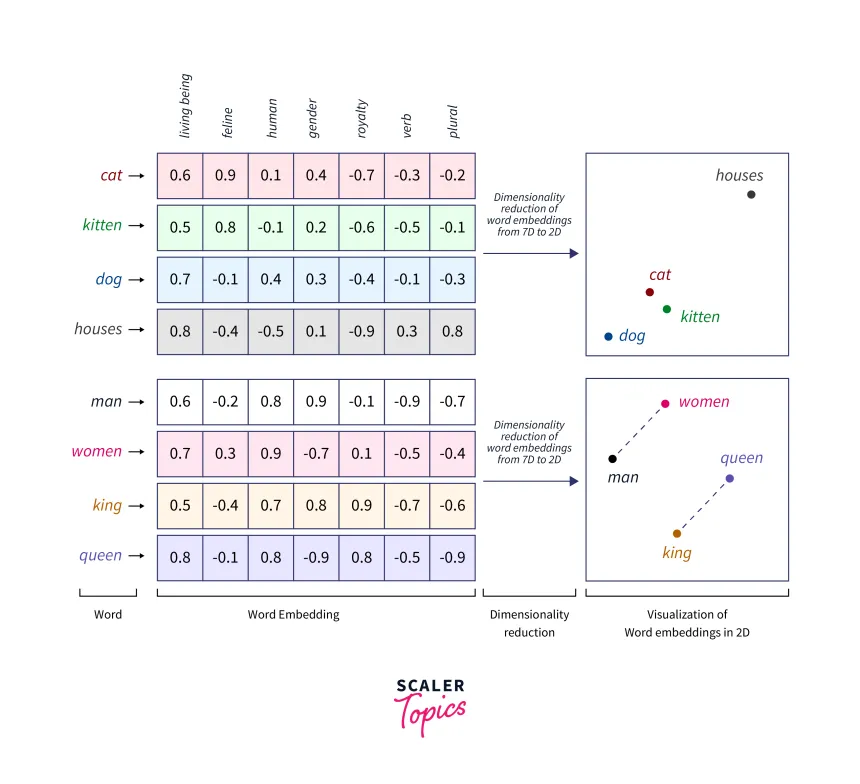
\includegraphics[width=0.8\linewidth]{imagenes/word-embedding-counting-model.png}
  \caption{Representación visual de un modelo basado en conteos para generar embeddings de palabras. Fuente: \url{https://www.scaler.com/topics/tensorflow/tensorflow-word-embeddings/}.}
  \label{fig:word_embedding_counting_model}
\end{figure}

\section{Espacios vectoriales y similitud semántica}

El espacio semántico \cite{worth_word_embeddings_2023} se define geométrica y algebraicamente como un espacio de $N$ dimensiones, donde $N$ representa el número de características. En las aplicaciones de aprendizaje automático para el \glsentrytext{pln}, estas características son típicamente palabras, n-gramas o frases completas.

Este espacio acota matemáticamente tanto el dominio del problema como el dominio de la solución. En el caso particular de los \textit{word embeddings}, las dimensiones son aprendidas por el propio modelo para asegurar que este exhiba ciertas propiedades; propiedades que son función de lo que se conoce como la \textbf{hipótesis distribucional}.

La hipótesis distribucional establece que las palabras que aparecen en contextos similares tienden a tener significados análogos. Para que el espacio vectorial refleje geométricamente esta propiedad sin que colapse analíticamente por culpa de tener miles o millones de características, no basta con usar métricas simples como el recuento de palabras. Es necesario transformar los datos basándose en el uso de \textbf{información latente}, logrando destilar el significado abstracto en unos pocos ejes temáticos.

Una vez que las palabras se han convertido en vectores y se han posicionado en este espacio latente optimizado, el siguiente paso natural es medir qué tan afines son sus significados. Esta similitud semántica se traduce matemáticamente en calcular la \textbf{distancia} geométrica que separa a ambos vectores.

A continuación, se detallan estos dos principios fundamentales para el funcionamiento profundo de los \textit{embeddings}.

\subsection{Información Latente}

% Aquí puedes adaptar la parte del texto que hablaba de "Latent information" (pasar del bag-of-words con perro/gato a los ejes latentes como "feline" o "mamífero")


\subsection{Métricas de Distancia}

% Aquí puedes adaptar la parte del texto de "Distance" (explicar la limitación de la distancia euclídea y por qué se normaliza con la distancia coseno)


\section{Paralelismo entre Espacio Semántico y Espacio de Hilbert}

Existe una analogía natural entre el espacio semántico clásico y el formalismo matemático de la mecánica cuántica.

En el \glsentrytext{pln} clásico, modelamos el significado de las palabras mapeándolas a vectores en un espacio vectorial real ($\mathbb{R}^n$). En la computación cuántica, operamos con estados cuánticos que "habitan" en un espacio vectorial complejo con producto interno, conocido formalmente como **Espacio de Hilbert** ($\mathcal{H}$).

Mientras que el espacio semántico clásico asigna vectores de características fijas, el Espacio de Hilbert ofrece un marco matemático mucho más rico. Los estados cuánticos en este espacio pueden existir en superposición y estar entrelazados, propiedades fundamentales que permiten representar la ambigüedad y la composición del lenguaje de una manera que los espacios vectoriales clásicos no pueden replicar eficientemente.

En el contexto del \glsentrytext{plnc}, la propuesta es mapear las palabras no a simples vectores reales, sino a estados cuánticos dentro de este Espacio de Hilbert. Esto permite que la gramática y el significado se combinen utilizando operaciones tensoriales y evolución unitaria, aprovechando la estructura exponencial del espacio de estados cuánticos para procesar el lenguaje.